% Theory
%
\chapter{Theory}\label{ch:theory}

This chapter covers the theoretical foundations and current state of technology essential for understanding this thesis work. The first section provides a basic introduction on what pulse compression radar is and how it generally works. The following two sections discuss the effects of nonlinearity and existing models that describe the nonlinearity exhibited by power amplifiers. Finally, predistortion is discussed - namely the general concept, how it can compensate for nonlinearity effects, and prominent predistortion algorithms in practice.

The goal of this chapter is not to cover the entire field of radar theory and nonlinearity at large, but rather to cover the key concepts and theory directly pertinent to this thesis work. This provides the reader context and prior knowledge to comprehend the work. 

\section{Pulse Compression Radar}

\section{Effects of Nonlinearity}\label{sec:nonlinearity_effects}

This section begins with a brief introduction to several concepts and equations paramount to understand nonlinearity and its effects. Firstly, a system can be called ``memoryless'' or ``static'' if its output depends solely on its current input value, and not on past input (or even output) values. Moreover, a memoryless system that is linear can be described by \cite{razavi}

\begin{equation}
  y(t) = \alpha \, x(t),
  \label{eq:memoryless_linear}
\end{equation}

where $y(t)$ is the output signal, $x(t)$ the input signal and $\alpha$ the constant gain of the system. Equation \eqref{eq:memoryless_linear} describes a linear relationship, as output is directly proportional to the input. 

On the contrary, a memoryless nonlinear system can be approximated by the power series, \cite{razavi}

\begin{equation}
  y(t) = \alpha_1 x(t) + \alpha_2 x^2(t) + \alpha_3 x^3(t) + \dotsb, 
  \label{eq:power_series}
\end{equation}

where it can be seen that the output $y(t)$ no longer shares a proportional change according to the input $x(t)$.  All electronic circuits are inherently nonlinear -- this is a fundamental truth of electronic engineering \cite{maas} -- as semiconductor materials used to build electronic components, such as transistors and diodes, do not scale their behaviour proportionally with input applied to them. The power amplifier of a transmission chain is of course not free from this truth, and existing models that attempt to describe its nonlinear behaviour are discussed in Section~\ref{sec:pa_models}. Whereas small signal operation of analogue and \gls{ac:rf} circuits can be approximated as linear, nonlinearities engender interesting effects that are not accounted for by the small-signal model. The remainder of this section elaborates on the most common phenomena observed for memoryless systems. To do so, we first describe a memoryless nonlinear system as \cite{razavi}

\begin{equation}
  y(t) \approx \alpha_1 x(t) + \alpha_2 x^2(t) + \alpha_3 x^3(t).
  \label{eq:memoryless_nonlinear}
\end{equation}

Equation \eqref{eq:memoryless_nonlinear} uses a third order polynomial; however as seen in \eqref{eq:power_series}, the power series can be extended for higher orders. The higher the order, the more precisely the equation can model the nonlinear behaviour of the system. The reader is cautioned that the effects of higher order nonlinearity terms and storage elements (introducing dynamic nonlinearity) are examined to determine whether \eqref{eq:memoryless_nonlinear} is a plausible representation \cite{razavi}. On that note, depending on operating region (bias and signal level), the degree of nonlinearity of a system can be characterised as either ``weakly'' or ``strongly'' nonlinear \cite{shi2000scs}. In practice, a power amplifier must operate well below saturation to be considered weakly nonlinear, wheareas a power amplifier operating close to the \qty{1}{\decibel} compression point (introduced in Subsection~\ref{sec:gain_compression}) is usually considered strongly nonlinear \cite{miehle}. The third order model is assumed to be a sufficient approximation for weakly nonlinear systems and is chosen for ease of instruction to explain the following effects. 

\subsection{Harmonics}

\begin{figure}[tb]
  \centering
  \begin{subfigure}[b]{0.9\textwidth}
    \centering
    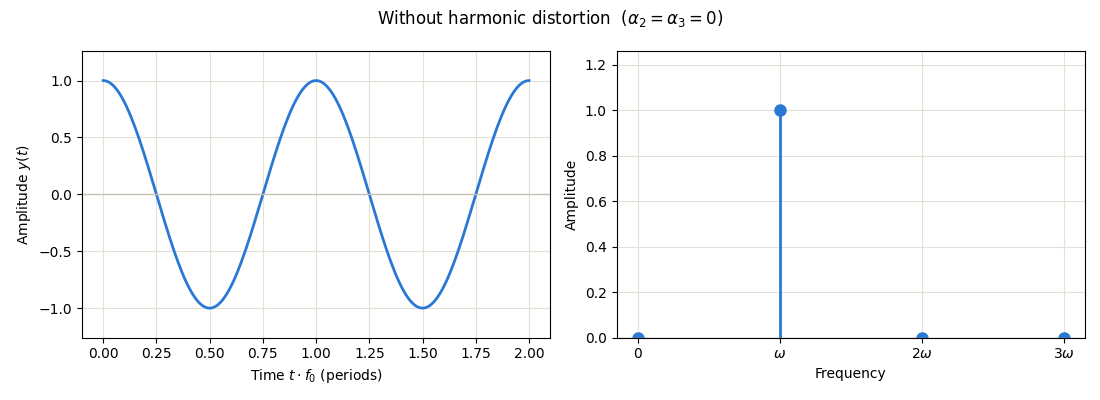
\includegraphics[width=\textwidth]{images/Without_harmonic_distortion}
    \caption{Without harmonic distortion, i.e.\ $\alpha_2 = 0$ and $\alpha_3 = 0$.}
    \label{fig:without_harmonic_distortion}
  \end{subfigure}
  \\[\bigskipamount]
  \begin{subfigure}[b]{0.9\textwidth}
    \centering
    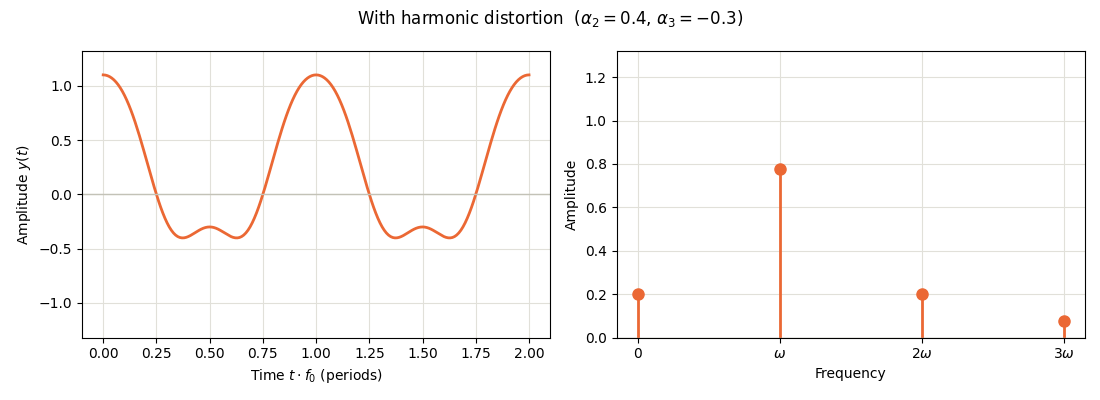
\includegraphics[width=\textwidth]{images/With_harmonic_distortion}
    \caption{With harmonic distortion, where $\alpha_2 = 0.4$ and $\alpha_3 = -0.3$.}
    \label{fig:with_harmonic_distortion}
  \end{subfigure}
  \caption{Simulation plots of the time and frequency domain, with and without
           harmonic distortion.}
  \label{fig:harmonic_distortion}
\end{figure}

The first phenomenon is harmonic distortion. When a sinusoid is applied to a nonlinear system, the output exhibits frequency components at integer multiples of the input frequency \cite{razavi} -- these are called harmonics. To demonstrate this, we apply a sinusoidal input of $x(t) = A\cos(\omega t)$ to equation \eqref{eq:memoryless_nonlinear}, then

\begin{align}
  y(t) &= \alpha_1 A\cos\omega t + \alpha_2 A^2\cos^2\omega t
          + \alpha_3 A^3\cos^3\omega t \label{eq:harmonic_expansion} \\
       &= \alpha_1 A\cos\omega t
          + \frac{\alpha_2 A^2}{2}\left(1 + \cos 2\omega t\right)
          + \frac{\alpha_3 A^3}{4}\left(3\cos\omega t + \cos 3\omega t\right) \\
       &= \frac{\alpha_2 A^2}{2}
          + \left(\alpha_1 A + \frac{3\alpha_3 A^3}{4}\right)\cos\omega t
          + \frac{\alpha_2 A^2}{2}\cos 2\omega t
          + \frac{\alpha_3 A^3}{4}\cos 3\omega t.
          \label{eq:harmonic_terms}
\end{align}

In \eqref{eq:harmonic_terms}, the first leftmost term is a dc term. The second term is the ``fundamental'', while the second and third terms are the second and third harmonics respectively. From the above expansion, we can make several observations. Firstly, the second-oder nonlinearity produces a dc term, as the first term contains the second-order coefficient $\alpha_2$. Secondly, each order $n$ of nonlinearity generates a harmonic at frequency $n \omega$. Lastly, the amplitudes of the second and third harmonic are proportional to $A^2$ and $A^3$ respectively, hence the $n$th harmonic grows proportional to $A^n$. 

Figure~\ref{fig:harmonic_distortion} depicts the harmonic distortion visually. In the ideal linear case shown in Figure~\ref{fig:without_harmonic_distortion}, there is a single peak located at the fundamental freqeuncy $\omega$. However, the nonlinear case of Figure~\ref{fig:with_harmonic_distortion} illustrates energy being distributed to the dc term and harmonics at frequencies $2 \omega$ and $3 \omega$ -- components that are created by nonlinearity.

\subsection{Gain Compression}\label{sec:gain_compression}

\begin{figure}[tb]
  \centering
  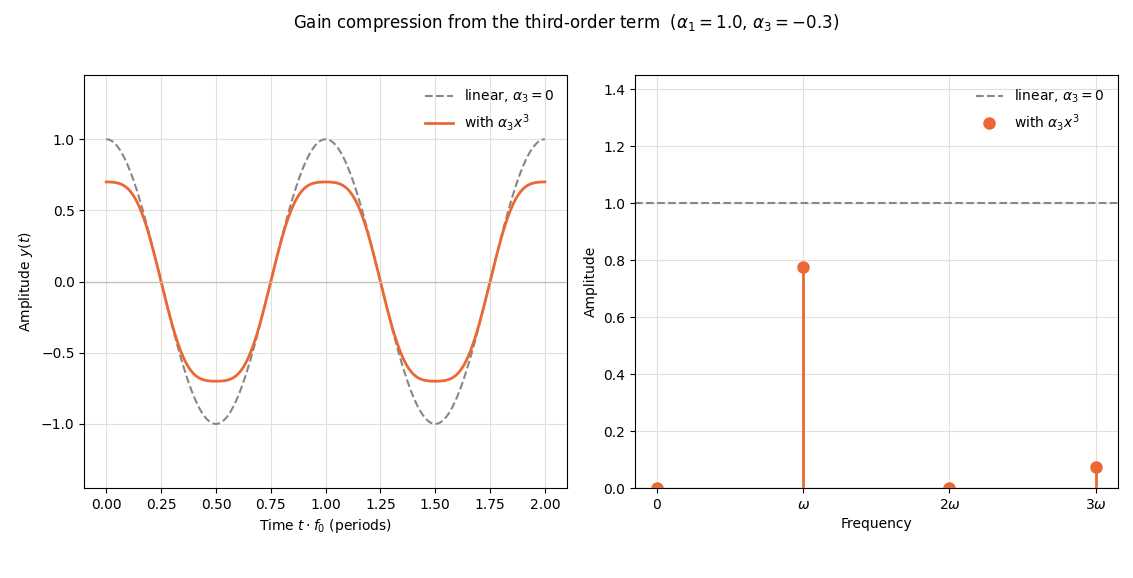
\includegraphics[width=0.9\textwidth]{images/Gain_compression}
  \caption{Gain compression in time and frequency domain caused by third-order nonlinearity with $\alpha_3 = -0.3$}
  \label{fig:gain_compression}
\end{figure}

Another effect of nonlinearity is gain compression -- where output gain decreases with increasing input amplitude \cite{razavi}. When looking at the fundamental term in \eqref{eq:harmonic_terms}, we see that the gain experienced by $A \cos \omega t$ is equal to $\alpha_1 + \frac{3\alpha_3 A^2}{4}$. This gain is dependent on the first and third-order coefficients $\alpha_1$ and $\alpha_3$. Analytically, if $\alpha_1 \alpha_3 > 0$, then $\alpha_1 x + \alpha_3 x$ overwhelms $\alpha_2 x$ for large $x$ regardless of the sign of $\alpha_2$, leading to an ``expansive'' characteristic. Inversely, for $\alpha_1 \alpha_3 < 0$, a ``compressive'' characteristic is seen for sufficiently large $x$. Figure~\ref{fig:gain_compression} graphically demonstrates the compressive behaviour for $y(t) = \alpha_1 x(t) + \alpha_3 x^3(t)$ -- simplifying to see the effect of the third-order nonlinearity term. As before, we see a harmonic produced at $3 \omega$, but more importantly, we see the third-order term compressing the peak amplitude of the output signal in both time and frequency domain. 

\begin{figure}[tb]
  \centering
  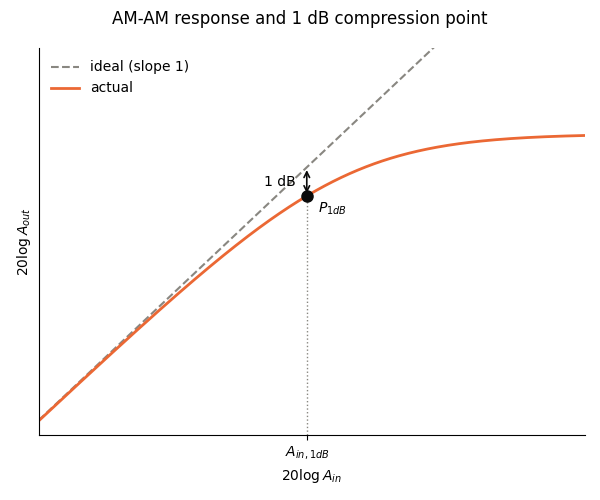
\includegraphics[width=0.9\textwidth]{images/P1dB}
  \caption{\qty{1}{\decibel} Compression Point}
  \label{fig:P1dB}
\end{figure}

This compression is quantified by the \qty{1}{\decibel} compression point \cite{razavi}. The \qty{1}{\decibel} compression point is defined as the point where the actual output gain deviates from the ideal output gain by \qty{1}{\decibel}, typically where the output begins to near saturation. The \qty{1}{\decibel} compression point is graphically depicted in Figure~\ref{fig:P1dB}.

To obtain the \qty{1}{\decibel} compression point mathematically, we equate the compressed gain of the fundamental term, $\alpha_1 + \frac{3\alpha_3 A_{\text{in}}^2}{4}$, to \qty{1}{\decibel} less than the ideal gain, $\alpha_1$. This results in equation \eqref{eq:1db_condition}.

\begin{equation}
  20\log\left|\alpha_1 + \frac{3}{4}\alpha_3 A_{\text{in,1dB}}^2\right|
  = 20\log\left|\alpha_1\right| - \qty{1}{\decibel} .
  \label{eq:1db_condition}
\end{equation}

From \eqref{eq:1db_condition}, the \qty{1}{\decibel} compression point with reference to input amplitude is

\begin{equation}
  P_{\text{\qty{1}{\decibel}}} = A_{\text{in,1dB}} = \sqrt{0.145\left|\frac{\alpha_1}{\alpha_3}\right|} .
  \label{eq:1db_point}
\end{equation}

\subsection{Desensitisation and Blocking}

Gain compression elucidated in Subsection~\ref{sec:gain_compression} has a further side-effect of decreasing system sensitivity - called ``desensitisation'' \cite{maas}. This means that weak received signals may be blocked by strong interference signals at different frequencies. This can occur when a receiver has to process a weak signal radiated from the transmitter alongside a strong signal emitted from another nearby transmitter \cite{wambacq}. Such decrease in sensitivity from saturation is another detrimental nonlinearity effect.   

\subsection{Intermodulation}

Another highly prevalent nonlinearity effect is intermodulation. This occurs when two signals with different frequencies $\omega_1$ and $\omega_2$ are applied to a nonlinear system, where the output then exhibits frequency components that are not harmonics. This phenomenon arises from the ``mixing'' (multiplication) of the two signals \cite{razavi}. The result is components generated at the new frequencies described by \eqref{eq:new_freqs} \cite{lee}.

\begin{equation}
  \omega = m\omega_1 \pm \omega_2.
  \label{eq:new_freqs}
\end{equation}

In \eqref{eq:new_freqs}, $\omega$ is the new frequency, where $\omega_1$ and $\omega_2$ are the original frequencies. $m$ and $n$ are positive integers including zero, and $m + n$ is eaual to the order of distortion. As such, using equation \eqref{eq:memoryless_nonlinear}, we determine that the second-order nonlinearity generates intermodulation products at $\omega_1 \pm \omega_2$ and third order nonlinearity at $2\omega_1 \pm \omega_2$ and $2\omega_2 \pm \omega_1$.

To understand the generation of new components mathematically, we take a two-tone input signal $x(t) = A_1\cos \omega_1 t + A_2\cos \omega_2 t$ and apply it to \eqref{eq:memoryless_nonlinear}, resulting in

\begin{equation}
\begin{split}
  y(t) &= \alpha_1(A_1\cos\omega_1 t + A_2\cos\omega_2 t)
          + \alpha_2(A_1\cos\omega_1 t + A_2\cos\omega_2 t)^2 \\
       &\quad + \alpha_3(A_1\cos\omega_1 t + A_2\cos\omega_2 t)^3 .
\end{split}
\label{eq:two_tone_input}
\end{equation}

If we expand the right-hand side of equation \eqref{eq:two_tone_input}, and discard dc terms, harmonics and second-order components at $\omega_1 \pm \omega_2$, we obtain the third-order intermodulation products in equations \eqref{eq:im3_a} and \eqref{eq:im3_b},

\begin{align}
  \omega = 2\omega_1 \pm \omega_2 :\quad
    &\frac{3\alpha_3 A_1^2 A_2}{4}\cos(2\omega_1+\omega_2)t
     + \frac{3\alpha_3 A_1^2 A_2}{4}\cos(2\omega_1-\omega_2)t
     \label{eq:im3_a} \\
  \omega = 2\omega_2 \pm \omega_1 :\quad
    &\frac{3\alpha_3 A_1 A_2^2}{4}\cos(2\omega_2+\omega_1)t
     + \frac{3\alpha_3 A_1 A_2^2}{4}\cos(2\omega_2-\omega_1)t
     \label{eq:im3_b},
\end{align}

along with the the fundamental components of equation \eqref{eq:fundamental_components}.

\begin{align}
  \omega = \omega_1,\ \omega_2 :\quad
    &\left(\alpha_1 A_1 + \frac{3}{4}\alpha_3 A_1^3
           + \frac{3}{2}\alpha_3 A_1 A_2^2\right)\cos\omega_1 t \nonumber \\
    &+ \left(\alpha_1 A_2 + \frac{3}{4}\alpha_3 A_2^3
           + \frac{3}{2}\alpha_3 A_2 A_1^2\right)\cos\omega_2 t
     \label{eq:fundamental_components}
\end{align}

\begin{figure}[tb]
  \centering
  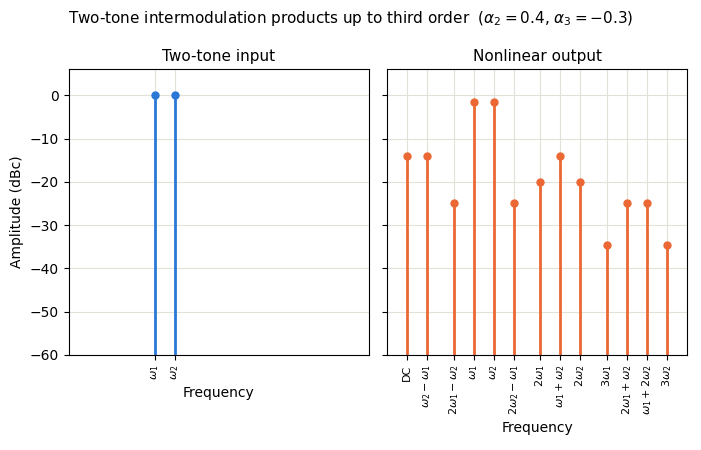
\includegraphics[width=0.9\textwidth]{images/Two-tone_intermodulation}
  \caption{Two-tone intermodulation products up to third-order with $\alpha_2 = 0,4$ and $\alpha_3 = -0,3$}
  \label{fig:two-tone_intermodulation}
\end{figure}

\begin{figure}[tb]
  \centering
  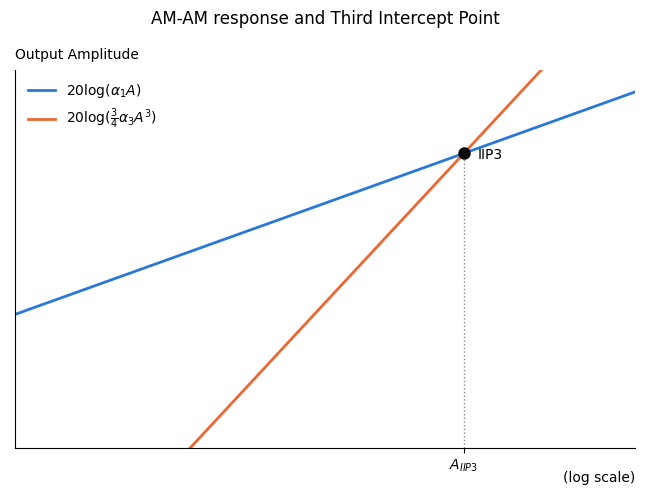
\includegraphics[width=0.9\textwidth]{images/Third-order_intercept}
  \caption{Third Order Intercept Point}
  \label{fig:third_order_intercept}
\end{figure}

Figure~\ref{fig:two-tone_intermodulation} graphically depicts the intermodulation products. The third-order intermodulation products at $2\omega_1 - \omega_2$ and $2\omega_2 - \omega_1$ are of particular interest, as they appear directly in the vicinity of $\omega_1$ and $\omega_2$.  These corrupt the transmitted signal - often lying within the transmission bandwidth. A common measure of the extent of third-order intermodulation products is the ``third intercept point'' ($IIP_3$) \cite{razavi}. This is defined as the point where the amplitude of the intermodulation products equals that of the fundamental tones at the output. This is demonstrated graphically in Figure~\ref{fig:third_order_intercept}. In practice, this point is usually never reached, as the output typically reaches saturation before this. 

To derive the third intercept point mathematically, the amplitude of the third-order intermodulation products in \eqref{eq:im3_a} and \eqref{eq:im3_b} can first be simplified for input tones of the same amplitude, i.~e. $A = A_1 = A_2$, to $\frac{3}{4}\alpha_3 A^3$. At the input at which this theoretical input third intercept point ($IIP3$) occurs, the uncompressed linear component $\alpha_1 A$ would equal the third order intermodulation product, resulting in

\begin{equation}
  \left|\alpha_1 A_{\text{IIP3}}\right|
  = \left|\frac{3}{4}\alpha_3 A_{\text{IIP3}}^3\right|,
  \label{eq:iip3_condition}
\end{equation}

solving for $A_IIP3$ yields the input third intercept point ($IIP3$)

\begin{equation}
  A_{\text{IIP3}} = \sqrt{\frac{4}{3}\left|\frac{\alpha_1}{\alpha_3}\right|}.
  \label{eq:iip3}
\end{equation}

\subsection{Phase Distortion}\label{sec:phase_distortion}

The final effect of nonlinearity we discuss is phase distortion. Sections~\ref{sec:nonlinearity_effects} has thus far only covered effects that involves nonlinear changes to the output amplitude with respect to input amplitude. This is commonly referred to as \gls{ac:am-am} conversion. However, most power amplifier circuits exhibit memory effects due to storage components such as capacitors and inductors, resulting in phase distortion from capacitive and inductive nonlinearities. This effect is commonly referred to as \gls{ac:am-pm} conversion \cite{miehle}. The cause behind \gls{ac:am-pm} conversion can be understood by taking the fundamental component from \eqref{eq:harmonic_terms} seen in \eqref{eq:fundamental_term} \cite{maas}.

\begin{align}
  \left(\alpha_1 A + \frac{3\alpha_3 A^3}{4}\right)\cos\omega t
  \label{eq:fundamental_term}
\end{align}

The input amplitude is denoted by $A$, while $\alpha_1$ and $\alpha_3$ are the first and third order coefficients respectively. The amplitude of equation \eqref{eq:fundamental_term} consists of the first order component $\alpha_1 A$ and the third order component $\frac{3\alpha_3 A^3}{4}$. Due to nonlinear capacitance, a phase difference can exist between these two components. The response is then a vector sum of two phasors illustrated in \eqref{eq:phasor_output}.

\begin{equation}
  V = \alpha_1 A + \frac{3}{4} \alpha_3 A^3 e^{j\theta} .
  \label{eq:phasor_output}
\end{equation}

In \eqref{eq:phasor_output}, $\alpha_1$ and $\alpha_3$ are again the first and third order coefficients respectively. The sum of the phasors is denoted $V$ and the phase difference between the first (linear) and third order term is denoted by $\theta$. As such, $\frac{3}{4} \alpha_3 A^3$ possesses a different phase from the linear component. Addition of the two phasors, linear and third order, leads to a phasor $V$ with a new angle. This new angle is dependent on variations in the input amplitude $A$, regardless of whether $\theta$ remains constant \cite{maas}. Hence, changes in input amplitude result in changes in output phase of the power amplifier, namely \gls{ac:am-am} conversion. This becomes more critical as the power amplifier is driven to higher input amplitudes into saturation, because the third order component increases commensurately with $A^3$.

\section{Power Amplifier Nonlinearity Models}\label{sec:pa_models}

Section~\ref{sec:nonlinearity_effects} described the effects that nonlinearity produces, but not how the nonlinear behaviour of a particular power amplifier is captured in a form suitable for simulation. Two broad approaches exist. Physical models derive the response from the geometry, material parameters and equivalent circuit of the transistor. Such models are accurate, but they are computationally expensive and demand device knowledge that manufacturers rarely disclose. Behavioural models instead treat the power amplifier as a black box and describe only the relationship between the input and output signal envelopes \cite{schreurs}. Because this thesis is concerned with system level effects rather than device physics, and because the parameters of a behavioural model can be extracted from the limited data published in manufacturer datasheets, behavioural models are the appropriate choice and form the subject of this section.

A memoryless behavioural model is fully characterised by two functions of the input envelope amplitude. The first, $A(r)$, returns the output amplitude for a normalised input amplitude $r$ and therefore describes \gls{ac:am-am} conversion. The second, $\Phi(r)$, returns the output phase shift and describes the \gls{ac:am-pm} conversion introduced in Subsection~\ref{sec:phase_distortion}. Each model below is accordingly presented as a pair of such expressions, whose coefficients are obtained by curve fitting against measured or datasheet characteristics. It should be noted that all models presented here are memoryless, and consequently reproduce neither frequency dependent behaviour nor the long term memory effects caused by thermal and bias network dynamics.

\subsection{Saleh Model}\label{sec:saleh_model}

The earliest and most widely cited behavioural model was proposed by Saleh for \gls{ac:twta} devices \cite{saleh}. Both conversion characteristics are expressed as rational functions of the input amplitude,

\begin{align}
  A(r)    &= \frac{\alpha_a r}{1 + \beta_a r^2},        \label{eq:saleh_amam} \\
  \Phi(r) &= \frac{\alpha_\phi r^2}{1 + \beta_\phi r^2}, \label{eq:saleh_ampm}
\end{align}

where $\alpha_a$ and $\beta_a$ determine the small signal gain and the saturation level of the amplitude characteristic, while $\alpha_\phi$ and $\beta_\phi$ determine the corresponding phase characteristic. The model requires only four parameters, which is a large part of its appeal. Its shortcoming is that it was derived for travelling wave tubes, whose compression characteristic differs markedly from that of a solid state device. Consequently the Saleh model represents \gls{ac:sspa} behaviour poorly \cite{fisher}, which motivated the models that followed.

\subsection{Ghorbani and Sheikhan Model}\label{sec:ghorbani_model}

Ghorbani and Sheikhan proposed a model specifically for \glspl{ac:sspa} \cite{ghorbani}. It retains the rational structure of the Saleh model but raises the input amplitude to a fitted exponent and adds a linear term, giving

\begin{align}
  A(r)    &= \frac{x_1 r^{x_2}}{1 + x_3 r^{x_2}} + x_4 r, \label{eq:ghorbani_amam} \\
  \Phi(r) &= \frac{y_1 r^{y_2}}{1 + y_3 r^{y_2}} + y_4 r. \label{eq:ghorbani_ampm}
\end{align}

The additional exponents $x_2$ and $y_2$ allow the sharpness of the transition into compression to be adjusted independently of the saturation level, and the linear terms $x_4 r$ and $y_4 r$ correct the slope in the small signal region. The eight parameters give the model appreciably more freedom than the Saleh model, and it fits solid state devices correspondingly better \cite{fisher}. The price is that the characteristic is known to ``roll over'' beyond the fitted range, that is, the predicted output amplitude begins to decrease once the input is driven past the region covered by the fitting data. This makes the model unreliable when extrapolated into deep saturation.

\subsection{Rapp Model}\label{sec:rapp_model}

The model proposed by Rapp is the one most commonly encountered in the \gls{ac:sspa} literature \cite{rapp}. Its \gls{ac:am-am} characteristic is

\begin{equation}
  A(r) = \frac{g\,r}{\left[1 + \left(\dfrac{g\,r}{A_{\text{sat}}}\right)^{2p}\right]^{\frac{1}{2p}}},
  \label{eq:rapp_amam}
\end{equation}

where $g$ is the small signal gain, $A_{\text{sat}}$ the saturated output amplitude and $p$ the smoothness factor, which controls how abruptly the characteristic transitions from the linear region into saturation. The structure of \eqref{eq:rapp_amam} is what distinguishes the model: the output tends towards $g\,r$ for small $r$ and asymptotically towards $A_{\text{sat}}$ for large $r$, so the characteristic is monotonic and saturates gracefully by construction rather than as a consequence of the fit. As $p \rightarrow \infty$ the model approaches an ideal limiter.

Rapp provided no \gls{ac:am-pm} expression, arguing that the phase conversion of a solid state amplifier is small enough to be neglected \cite{rapp}. That assumption does not hold for the devices of interest here, and Honkanen and H\"aggman subsequently supplied a phase characteristic intended to be used alongside \eqref{eq:rapp_amam} \cite{honkanen}. Their expression describes a phase shift that descends with increasing drive level, but it is bounded above by zero degrees, so it cannot represent a device whose phase shift is positive at low drive. Fisher and Al-Sarawi addressed this by introducing an additional offset parameter, which shifts the whole characteristic and thereby admits positive phase shifts \cite{fisher}.

\subsection{Later Refinements}\label{sec:later_pa_models}

Two further refinements are relevant. White, Burr and Javornik proposed a model formulated as a combination of exponential terms, reporting improved accuracy over the Saleh, Ghorbani and Sheikhan, and Rapp models \cite{white}. Fisher and Al-Sarawi were unable to reproduce those results using the equation as published, and concluded that the expression contains a typographical error; with the corrected form the reported accuracy is recovered \cite{fisher}. This is worth noting, as it illustrates that a published behavioural model cannot simply be adopted without verification against the data it claims to fit.

O'Droma, Meza and Lei proposed a modified Saleh model developed for \gls{ac:ldmos} based amplifiers \cite{odroma}. It retains the compact rational form of the original but reshapes the amplitude characteristic so that it follows a solid state device more closely, and it achieves the best fit of all models considered when measurement data extending into saturation is available \cite{fisher}.

\subsection{Model Comparison and Selection}\label{sec:pa_model_selection}

Fisher and Al-Sarawi compared the above models by fitting each to the same measured device data and evaluating the \gls{ac:nmse} of the resulting \gls{ac:am-am} characteristic \cite{fisher}. Their results are reproduced in Table~\ref{table:pa_model_nmse}, where a more negative figure indicates a closer fit.

\begin{table}[tb]
  \caption{\gls{ac:am-am} modelling accuracy of behavioural power amplifier models, after
           Fisher and Al-Sarawi \cite{fisher}.}
  \label{table:pa_model_nmse}
  \begin{center}
    \begin{tabular}{l|r}
      Model & \gls{ac:nmse} (\unit{\decibel}) \\
      \hline
      Saleh \cite{saleh}                        & $-27.13$ \\
      Ghorbani and Sheikhan \cite{ghorbani}     & $-35.44$ \\
      Rapp \cite{rapp}                          & $-42.33$ \\
      White et al.\ \cite{white}                & $-36.95$ \\
      White et al., corrected \cite{fisher}     & $-44.00$ \\
      Modified Saleh \cite{odroma}              & $-48.54$ \\
    \end{tabular}
  \end{center}
\end{table}

Two conclusions follow. Firstly, the Saleh model is clearly the weakest for solid state devices, which is consistent with its origin as a travelling wave tube model. Secondly, the ranking depends on how far the fitting data extends. When only data below saturation is available, which is the usual situation when parameters are extracted from a datasheet, the Rapp model of \eqref{eq:rapp_amam} extrapolates into the saturation region more reliably than the models that fit the measured range more tightly \cite{fisher}. When measurement data extending into saturation is available, the modified Saleh model is the most accurate in that region.

This distinction matters for the present work. The power amplifier of the \gls{ac:sspa} chain under investigation is to be driven towards saturation deliberately, so the behaviour of a model beyond the fitted range is as important as its accuracy within it. The Rapp model of \eqref{eq:rapp_amam}, together with the phase characteristic of Honkanen and H\"aggman and the offset of Fisher and Al-Sarawi, is therefore adopted as the primary nonlinearity model in this thesis, with the modified Saleh model retained as a comparison once laboratory measurements covering the saturation region are available. The selection is revisited in Chapter~\ref{ch:concept_and_design}.

\section{Predistortion}